% !TeX root = Phase2.tex
% !TeX program = pdflatex
% Standalone submission source. Compile this file to produce Phase2.pdf.
% Bibliography is embedded; no separate BibTeX run is required.
\documentclass[11pt,a4paper]{article}
\usepackage[utf8]{inputenc}
\usepackage[T1]{fontenc}
\usepackage{lmodern}
\usepackage[margin=1in]{geometry}
\usepackage{titlesec}
\usepackage{enumitem}
\usepackage{hyperref}
\usepackage{xcolor}
\usepackage{graphicx}
\usepackage{subcaption}
\usepackage[authoryear,round]{natbib}
\renewcommand{\bibsection}{} % Explicit reference headings are provided below.
\usepackage{microtype}
\usepackage{float}
\usepackage{booktabs}
\usepackage{tabularx}
\usepackage{array}
\setlength{\parskip}{0.35em}

% --- Custom Styling for Academic Polish ---
\definecolor{tuedark}{HTML}{1E293B}
\definecolor{tuegreen}{HTML}{16A34A}

\titleformat*{\section}{\large\bfseries\color{tuedark}}
\titleformat*{\subsection}{\bfseries\color{tuedark}}
\hypersetup{
    colorlinks=true,
    linkcolor=tuedark,
    urlcolor=tuegreen,
    citecolor=tuegreen
}

% --- Cover/Metadata Setup ---
\title{\textbf{Group Q: Phase 2 Report}\\[0.5em]\Large Research Roots\\[0.3em]\large Author revision copy -- not for submission}

\author{\textbf{Group Q} \\\\
Course: 5ARF0 Ethics of AI: Theory and Practice \\
Eindhoven University of Technology}
\date{23 October 2026}



% BEGIN embedded assignment2-wordcounts.tex
\newcommand{\Bwordcount}{119}
\newcommand{\Cwordcount}{1644}
\newcommand{\Dwordcount}{295}
\newcommand{\Fwordcount}{385}

% END embedded assignment2-wordcounts.tex


\begin{document}

\maketitle
\vspace{0.6cm}
% Member details copied from the existing samplemscthesis.tex cover.
\begin{center}
\small
\renewcommand{\arraystretch}{1.2}
\begin{tabularx}{\textwidth}{@{}>{\raggedright\arraybackslash}p{0.29\textwidth}>{\raggedright\arraybackslash}p{0.14\textwidth}X@{}}
\toprule
\textbf{Name} & \textbf{Student ID} & \textbf{Email} \\
\midrule
Yehao Chen & 2216655 & \href{mailto:y.chen13@student.tue.nl}{\nolinkurl{y.chen13@student.tue.nl}} \\
Dennis de Hoon & 1732773 & \href{mailto:d.b.a.d.hoon@student.tue.nl}{\nolinkurl{d.b.a.d.hoon@student.tue.nl}} \\
Gerald Tobenna Eluagu & 2419289 & \href{mailto:g.t.eluagu@student.tue.nl}{\nolinkurl{g.t.eluagu@student.tue.nl}} \\
Peng Wang & 2342944 & \href{mailto:p.wang1@student.tue.nl}{\nolinkurl{p.wang1@student.tue.nl}} \\
\bottomrule
\end{tabularx}
\end{center}
\vspace{0.6cm}
\noindent\textit{Team revision copy: Sections B and C have been aligned with the two-tree research-discovery design. Section C now includes deployment, cold start, replication choices, governance and evaluation. Dennis's Section D remains for his final revision. Gerald coordinates the other components; Sections F and G still show the legacy self-assessment example, and H requires contributor records. The editorial checklist at the end is for team review and must be removed before submission.}

\medskip
\noindent\small Word counts use TeXcount narrative-text counts, excluding headings, citations, references, captions and editorial notes. Recount after further edits.\normalsize

\thispagestyle{empty}
\clearpage
\pagestyle{plain}
% A. PROJECT TITLE
% =========================================================================
\section*{A. Project Title}
\addcontentsline{toc}{section}{A. Project Title}

\noindent\textbf{Research Roots: Finding Related TU/e Research and Reusable Resources}
% =========================================================================
% B. PUBLIC SUMMARY
% =========================================================================
% Gerald: review the updated public summary against the final product name and shared demonstration.
\section*{B. Public Summary}
\addcontentsline{toc}{section}{B. Public Summary}
\noindent\textit{Word count: \Bwordcount / 150}\par\medskip


\noindent Research Roots would help TU/e students and researchers find existing work and resources while planning a study. Users describe their question and methods, then explore two trees: one shows connections to earlier research; the other highlights possible differences to investigate. Each connection leads to a source that users can check. The aim is to make useful knowledge, equipment and potential collaborators easier to discover, creating opportunities to reuse resources before committing to a new experiment. Researchers remain free to pursue replication and disregard suggestions. The main challenges are incomplete records, misleading connections and protecting unpublished ideas. A proposed pilot would test whether the tool helps users make better planning decisions and whether reuse leads to measurable resource savings.

\clearpage

% =========================================================================
% C. COMPREHENSIVE SUMMARY
% =========================================================================
% Section C substantively revised from the author-provided design and verified sources on 23 October 2026.
\section*{C. Comprehensive Summary}
\addcontentsline{toc}{section}{C. Comprehensive Summary}
\noindent\textit{Word count: \Cwordcount / 2000}\par\medskip

\subsection*{Problem Definition and Objective(s)}

A student planning a study may find publications on the same topic while overlooking a useful method, dataset or piece of equipment in another TU/e department. The TU/e research portal already contains publications, projects, equipment and facilities \citep{tueportal}; the problem we address is discovering relevant connections before the student knows the right author or search term. Its extent at TU/e still requires local investigation. We therefore propose a design strategy for research discovery rather than claim that researchers routinely waste resources.

Research Roots would let students and researchers describe a planned study and explore related work through a Similarity Tree and a Distinctiveness Tree. The intended change is to make potential reuse visible while research plans remain open to revision. A LiDAR study, for example, might benefit from a sensing method used for another application. Researchers would still need to check whether the method transfers and whether the associated resources are available.

Students gain a starting point for discussion with supervisors; researchers can discover potential collaborators and resources. Librarians would help with discovery and metadata, equipment managers would confirm access conditions, and data stewards would advise on sharing. Their participation is necessary: a matching record cannot establish permission or suitability for reuse. The tool would support planning, without assessing eligibility for funding or deciding whether a project deserves to proceed.

\subsection*{Background of Current Approaches and Knowledge}

The research portal provides an institutional starting point, while OpenAlex could supplement the published literature beyond TU/e \citep{openalex2026}. These sources serve different purposes: wider literature contextualises a research question; institutional records help locate local expertise and resources. Neither establishes complete coverage of ongoing or confidential work. Pure and Research Cockpit should also be distinguished. Pure offers research-information services; TU/e's Research Cockpit supports processes including data management and ethical applications \citep{pureapi,tuerdm}. A link from an existing workflow would not imply access to its underlying data.

SPECTER provides a research basis for representing scientific documents through citation-informed learning \citep{cohan2020}. SciRepEval evaluates representations across different scientific tasks \citep{singh2023}. Neither establishes the accuracy of matching short TU/e project descriptions. Our technical question is therefore whether semantic retrieval adds useful connections beyond keyword search in this setting. The design must also explain those connections, disclose missing information and permit correction; finding similar text alone does not establish scientific relevance.

\subsection*{Plan of Approach / Design Strategy}

\paragraph{Two trees and the knowledge boundary.}
Users would enter a research question, method and relevant resource needs, then choose which aspects to prioritise. Keyword and semantic retrieval would search permitted records. The Similarity Tree would group connections by question, method or resource, helping researchers identify evidence and possible reuse. The Distinctiveness Tree would describe differences from those records and questions worth investigating. Future directions belong within this second tree, avoiding a separate third output. Each branch would open a source card with the original record, the reason for the connection, its update information and any relevant missing fields. We would avoid a single similarity or novelty percentage that conceals these different relationships.

Matt Might's illustrated guide describes research as building knowledge towards a boundary and contributing beyond it \citep{might}. We use this as a visual metaphor: existing work supports the researcher's foundation, while differences suggest questions to investigate. Our interface can represent only the selected records, not the boundary of all human knowledge. Adding an overlooked paper could change an apparent difference. The visualisation should make this dependence clear rather than present an empty region as proof of a research gap.

\paragraph{Replication and researcher choice.}
At input, researchers could indicate whether a module aims to explore a new question, reproduce a result or identify reusable resources. Someone conducting replication could disable distinctiveness suggestions for that module while retaining references and method connections. They could accept, correct or disregard recommendations without having to justify the study to the system. This choice concerns optional advice; it does not bypass experimental safety, ethical review or access restrictions. Similarity can be valuable evidence for replication, and the same method may answer a different question.

\paragraph{Institutional deployment and cold start.}
The proposed deployment is a TU/e-managed web service on a university subdomain, using institutional hosting such as Azure if approved. SURFconext single sign-on would avoid a separate password account. Its guidance recommends minimal attribute disclosure; for returning accounts we would request a persistent pseudonymous OpenID Connect \texttt{sub} identifier \citep{surfattributes}. The application would separately manage permissions for private drafts and shared records. Linking an account to Pure would require an approved mapping and user verification; we would not assume that \texttt{eduPersonPrincipalName} is a persistent cross-system key. Hosting, security review, data-protection assessment and operational ownership would be agreed with university staff before deployment. These arrangements are proposed, not secured approvals.

Cold start has two distinct forms. First, the collection must be useful before users contribute descriptions. We would seed a limited pilot with permitted Pure/portal titles, abstracts, affiliations and equipment descriptions, recording provenance and update dates. The Pure API documentation confirms that access depends on permissions and sharing configuration \citep{pureapi}. Access to grants or unpublished projects cannot be assumed. We would begin with records from two departments, check coverage with their researchers and expand after correcting omissions.

Second, new users may have no publication history. Manual descriptions must therefore support the complete basic search. Users with a Pure profile could optionally review imported research information as context, then correct or reject it. Historical publications would not define their current interests. A short survey would investigate discovery needs and willingness to share; it would inform the design rather than substitute for missing research records.

For equipment omitted from abstracts, researchers or equipment managers could confirm resource tags. Integration with booking systems remains a later option: reservations do not establish actual use or suitability for another study. Automatically inferring methods and citations from bookings would introduce unsupported claims and additional personal-data processing. We would first test whether confirmed equipment descriptions meet the discovery need. The tool could direct users towards existing institutional workflows without becoming a mandatory stage in DMP approval.

\paragraph{Values, participation and governance.}
Value Sensitive Design (VSD) connects conceptual, empirical and technical investigations \citep{friedman2008,vsdlab}. Conceptually, we would examine sustainability, privacy, fairness, explicability and researcher autonomy, including people whose work appears in results but who never use the tool. Empirically, interviews and mock-up walkthroughs with researchers, students and support staff would examine useful connections, unacceptable disclosures and maintenance burdens. Technically, these findings would shape access controls, source explanations and sharing choices. Research with participants or personal data would follow TU/e's ethical-review procedures \citep{tueethics}.

A concrete conflict concerns discovery versus confidentiality. A researcher may want others to find a reusable setup while protecting an unpublished hypothesis. Using VSD value scenarios, we would compare sharing a full description, sharing confirmed resource tags, and keeping the draft private. Participants would explain benefits and objections; the team would document its choice, affected parties and reasons, then test the revised interface with them. Our proposed default is a private draft with separately chosen sharing and contact preferences. This sacrifices some discovery coverage to protect control over unfinished work; stakeholder review would assess whether narrower sharing remains useful.

Withdrawal would remove a voluntarily shared summary from active discovery and initiate removal from derived indexes and caches. Saved views controlled by the service would hide withdrawn content and indicate that it is unavailable. This cannot guarantee deletion of external downloads or remove independently public publications. Approved retention arrangements would cover backups and necessary logs. TU/e's RDM framework defines research-data responsibilities \citep{tuerdm}. For this service, we propose a named owner coordinating corrections and withdrawals, with source and equipment owners maintaining their records under agreed responsibilities.

\paragraph{Evaluation and route towards impact.}
The pilot would compare the current portal with the proposed interface using equivalent planning tasks, balancing task order to reduce practice effects. Domain experts would judge the relevance of top results and whether explanations accurately reflect their sources. Relevance would be reported as the proportion of reviewed results judged useful; explanation errors would be claims unsupported by the linked records. We would record time to find a useful connection, missed relevant records and whether users understand the coverage limits. Results would be examined across departments and users with or without publication histories, so stronger metadata coverage does not conceal poor support for newcomers.

Users could flag an incorrect connection or outdated record. The service owner would check the source, distinguish metadata errors from retrieval or explanation errors, revise the relevant component, and repeat the affected tasks before releasing the change. A rejected suggestion would not automatically become a training label. Keeping a versioned correction record would make improvements inspectable and help determine whether errors recur.

Environmental impact requires a further chain of action: a researcher identifies a resource, its owner confirms access and suitability, the researcher changes the plan, and the resulting inputs are measured. We would compare the original and revised plans for the same scientific objective and quality requirements. Electricity and material use would be reported separately, including additional preparation, transport or cleaning where relevant and the platform's own computing costs. Uncertain estimates would remain identified as estimates. Follow-up would establish whether a suggested match actually led to reuse; clicks or accepted suggestions would not count as resource savings. Valuable replication would remain a scientific objective rather than an avoided cost.

\subsection*{Comparison to Alternatives}

Our Phase 1 self-assessment concept acted after an activity was defined, requiring resource measurements and reference data. Research Roots moves the intervention earlier, when finding an existing method or resource might still change the plan. It complements rather than replaces subsequent footprint assessment.

Improved portal filters and librarian-supported keyword searches are a simpler alternative. We would retain them as the baseline and fallback because they avoid some model and maintenance costs. Semantic retrieval is worth pursuing only if the pilot finds useful connections that this baseline misses, without unacceptable explanation errors or burdens. University-wide automatic profiling is another option, but requires broader permissions and risks exposing unfinished work. The limited, optional-import approach gives priority to a testable service with clear responsibilities. Its contribution is a strategy for informed research planning; effectiveness and net environmental benefit still require evaluation.


% =========================================================================
% D. RESPONSIBLE INNOVATION PROJECT STATEMENT
% =========================================================================
\clearpage
% AUTHOR TODO -- Dennis: keep existing transparency/coverage discussion; develop one concrete value conflict, withdrawal, autonomy and feedback handling; max 1000 words.
\section*{D. Responsible Innovation Project Statement}
\noindent\textit{Word count: \Dwordcount / 1000}\par\medskip
This statement examines transparency, bias and reliability in the proposed research-matching tool. The measures below address the values identified in our Value Sensitive Design approach: explicability, fairness and researchers' control over results \citep{friedman2008}.

\subsection*{Transparency}
Users submit a research description and receive potentially relevant previous work. They need to understand why each source was selected and be able to check the AI's explanation. We propose the following measures:
\begin{itemize}[leftmargin=*]
    \item \textbf{Source transparency:} Each source should include its title, authors, publication year and a link to the original source, with additional information where available. Researchers can then verify the sources rather than rely solely on the AI.
    \item \textbf{Explanation of relevance:} Each source should have a short explanation of why it was selected, identifying similarities in research questions, methods or other relevant aspects.
\end{itemize}

\subsection*{Bias and coverage}
The tool's results may be biased by the sources available to it. For example, access limited to journal articles or English-language sources could cause researchers to miss relevant previous work. We propose the following measures to reduce this risk:
\begin{itemize}[leftmargin=*]
    \item \textbf{Database coverage:} Users should be able to see which databases the tool searches, so that they understand its limitations.
    \item \textbf{Search strategies:} Where possible, the search should use synonyms, similarities across disciplines and different terminology.
    \item \textbf{User input:} Users should be able to adjust their search query, giving them more control when the AI encounters limitations.
\end{itemize}

\subsection*{Interpreting results and future work}
Our design aims to make results easy to interpret through an interface that provides sources and explains their relevance. Future work could help researchers identify ways to refine their research or investigate differences from earlier work. Previous work on the same topic does not necessarily mean that a researcher should abandon a project: there may still be useful differences to explore. In such cases, the tool could also help researchers consider better use of research resources.


% =========================================================================
% E. REFERENCE LIST
% =========================================================================
\clearpage
\section*{E. Reference List}
\addcontentsline{toc}{section}{E. Reference List}

\begin{thebibliography}{99}

\bibitem[Cohan et~al.(2020)]{cohan2020}
Cohan, A., Feldman, S., Beltagy, I., Downey, D., \& Weld, D. (2020).
SPECTER: Document-level representation learning using citation-informed transformers.
\emph{Proceedings of the 58th Annual Meeting of the Association for Computational Linguistics}, 2270--2282.
\url{https://doi.org/10.18653/v1/2020.acl-main.207}

\bibitem[Friedman et~al.(2008)]{friedman2008}
Friedman, B., Kahn, P. H., Jr., \& Borning, A. (2008).
Value sensitive design and information systems.
In K. E. Himma \& H. T. Tavani (Eds.), \emph{The handbook of information and computer ethics}. Wiley.
\url{https://doi.org/10.1002/9780470281819.ch4}

\bibitem[Might(n.d.)]{might}
Might, M. (n.d.).
\emph{The illustrated guide to a Ph.D.}
\url{https://matt.might.net/articles/phd-school-in-pictures/}

\bibitem[OpenAlex(n.d.)]{openalex2026}
OpenAlex. (n.d.).
\emph{Works overview}.
Retrieved October 23, 2026, from
\url{https://help.openalex.org/data/works/}

\bibitem[Singh et~al.(2023)]{singh2023}
Singh, A., D'Arcy, M., Cohan, A., Downey, D., \& Feldman, S. (2023).
SciRepEval: A multi-format benchmark for scientific document representations.
\emph{Proceedings of the 2023 Conference on Empirical Methods in Natural Language Processing}, 5548--5566.
\url{https://doi.org/10.18653/v1/2023.emnlp-main.338}

\bibitem[SURF(n.d.)]{surfattributes}
SURF. (n.d.).
\emph{Attribute best practice}.
\url{https://servicedesk.surf.nl/wiki/spaces/IAM/pages/128910241/Attribute+best+practice}

\bibitem[TU/e(n.d.-a)]{pureapi}
Eindhoven University of Technology (TU/e). (n.d.-a).
\emph{Pure API documentation}.
\url{https://pure.tue.nl/ws/api/documentation/index.html}

\bibitem[TU/e(n.d.-b)]{tueportal}
Eindhoven University of Technology (TU/e). (n.d.-b).
\emph{Research portal}.
\url{https://research.tue.nl/en/}

\bibitem[TU/e(2026a)]{tueethics}
Eindhoven University of Technology (TU/e). (2026a, October 15).
\emph{Ethical approval}.
\url{https://rdm.tue.nl/docs/before-research/ethical-approval/}

\bibitem[TU/e(2026b)]{tuerdm}
Eindhoven University of Technology (TU/e). (2026b, June 9).
\emph{TU/e RDM framework policy}.
\url{https://rdm.tue.nl/docs/intro/tue-policy/}

\bibitem[VSD Lab(n.d.)]{vsdlab}
VSD Lab. (n.d.).
\emph{About VSD}.
\url{https://vsdesign.org/vsd/}

\end{thebibliography}


\clearpage
% =========================================================================
% F. USER NARRATIVE
% =========================================================================
% AUTHOR TODO -- Gerald: replace old energy-calculator scenario with current two-tree journey; max 500 words.
\section*{F. User Narrative}
\addcontentsline{toc}{section}{F. User Narrative}
\noindent\textit{Word count: \Fwordcount / 500}\par\medskip

\noindent Dr. Alex, a postdoctoral researcher at Eindhoven University of Technology, is designing a new fabrication run of lithium-ion battery electrode samples within a TU/e laboratory building. Eager to lower total electricity and material waste without changing the scientific parameters that make the batch valid, Alex logs onto the AI-Supported Sustainability Self-Assessment (ENSU) web portal from his laptop or phone.

On the home dashboard, Alex selects "1. I want to Assess", initiating a 5-step evaluation process. Rather than selecting fixed checkboxes, Alex inputs a plain-text description: "I make lithium-ion battery electrode samples. I want to minimize material loss and electricity use while preserving our existing electrochemical testing requirements." The language model interprets the description and proposes an activity classification: "This appears to be a laboratory battery-sample activity." Alex clicks "Confirm activity", advancing to the data input sheet.

Alex completes the project fields based on a prior set of data: 6 fabrication attempts yielding 5 valid samples, consuming 60 kWh of meter-tracked laboratory electricity and 1.2 kg of starting materials. The system asks a follow-up question regarding what constitutes a valid sample. Alex types: "A valid sample passes our electrochemical test and safety checks."

Upon confirming the fields, the tool runs its step-by-step calculation engine and outputs an initial evaluation profile. Rather than showing an aggregated green score or compliance badge, the interface reports separate resource-use indicators: electricity use of 12 kWh per valid sample, which is 2 kWh above Alex's personal sustainability target of 10 kWh. Beneath the values, a targeted suggestion appears: "Pilot a process change that reduces failed samples; record electricity, starting material, valid samples, and test results for the whole batch." Alex clicks "Plan pilot", exits the interface, and tests the proposed process change in the lab.

A week later, Dr. Alex returns to the ENSU web portal. He navigates to "My History" under the "Query" module, and logs the pilot outcomes: 6 attempts, 6 valid samples, 54 kWh, and 1.1 kg of material. The comparison dashboard updates instantly, using visual bars to compare the two batches: batch electricity dropped by 6 kWh, material consumption fell by 0.1 kg, and electricity use reached 9 kWh per valid sample, meeting Dr. Alex's original electricity-use target. Alex saves the session privately to his personal archive, using the recorded comparison to review his research plan.



\clearpage
% AUTHOR TODO -- Gerald: replace old screenshots; exactly one A4 page corresponding to revised F.
\section*{G. Visual Representation of Mock-up}
\addcontentsline{toc}{section}{G. Visual Representation of Mock-up}

\begin{figure}[H]
    \centering
    \captionsetup[subfigure]{font=scriptsize,skip=2pt}
    % Row 1
    \begin{subfigure}{0.48\linewidth}
        \centering
        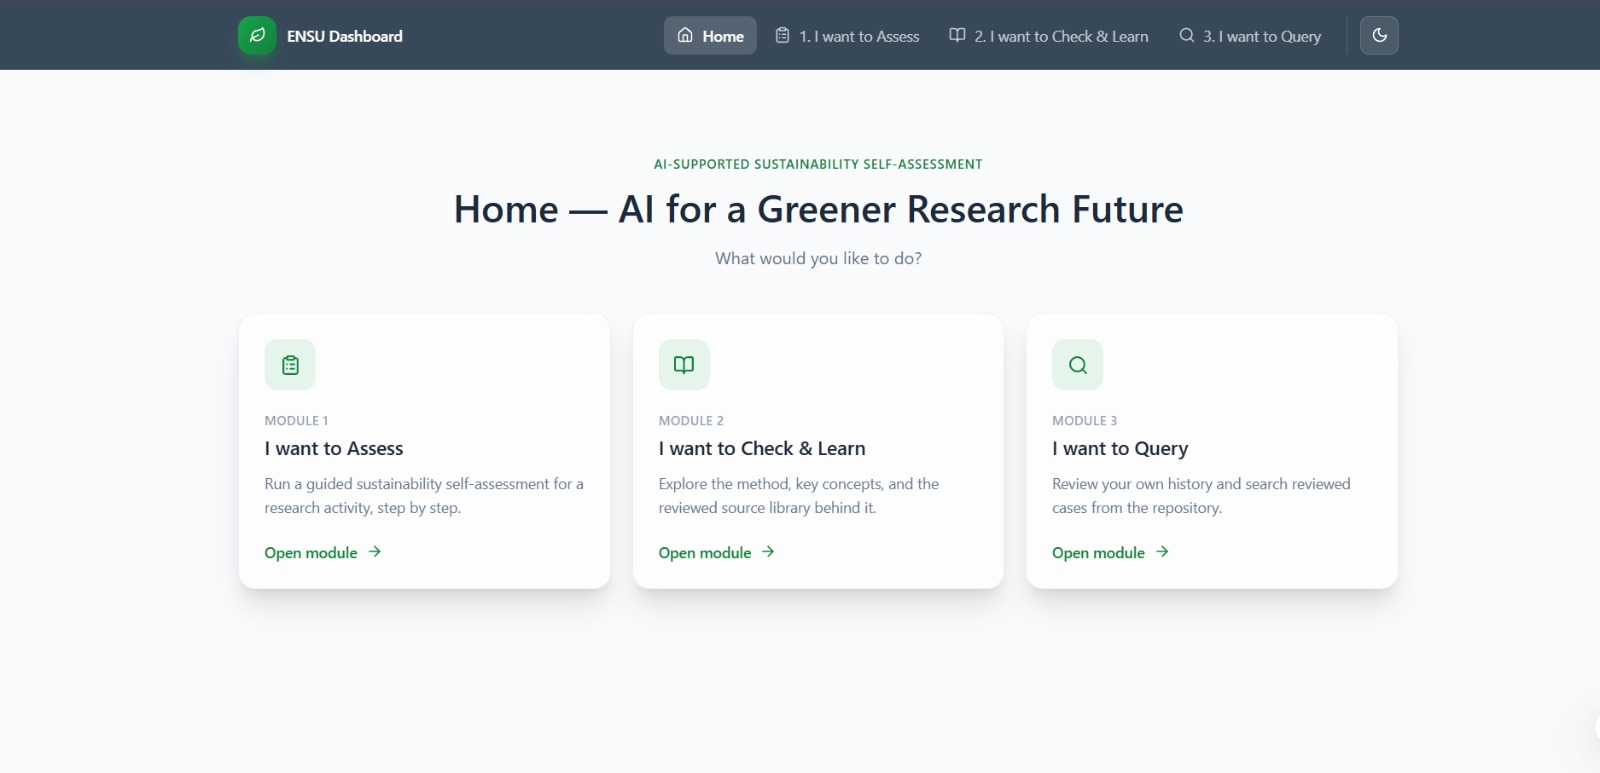
\includegraphics[width=\linewidth,height=0.115\textheight,keepaspectratio]{assets/images/phase2/01-home-light.jpeg}
        \caption{Home page - Light Mode}
    \end{subfigure}
    \hfill
    \begin{subfigure}{0.48\linewidth}
        \centering
        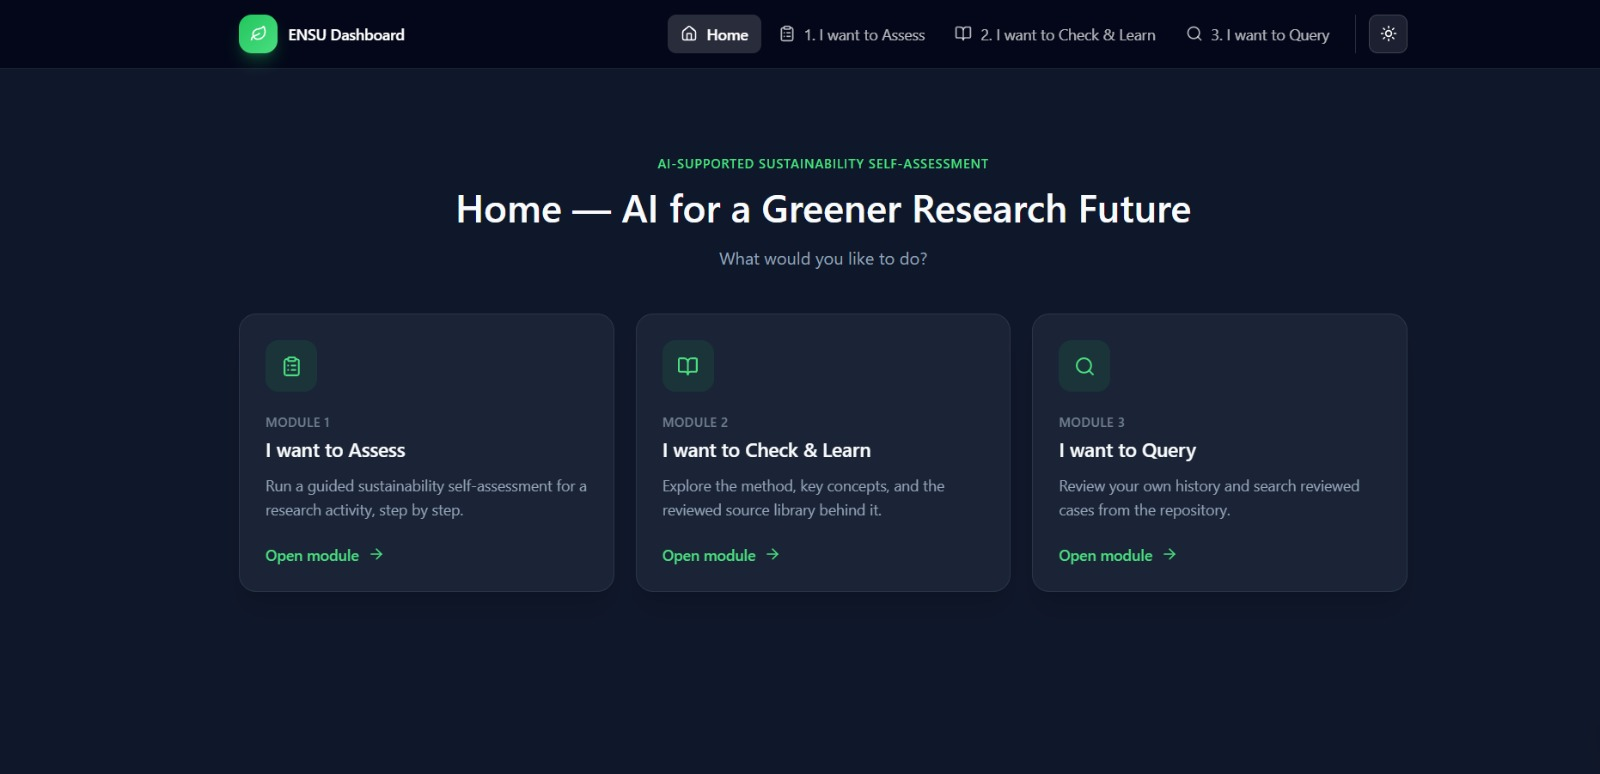
\includegraphics[width=\linewidth,height=0.115\textheight,keepaspectratio]{assets/images/phase2/02-home-dark.jpeg}
        \caption{Home page - Dark Mode}
    \end{subfigure}

    \vspace{0.12cm} % Tightly controls vertical spacing between rows

    % Row 2
    \begin{subfigure}{0.48\linewidth}
        \centering
        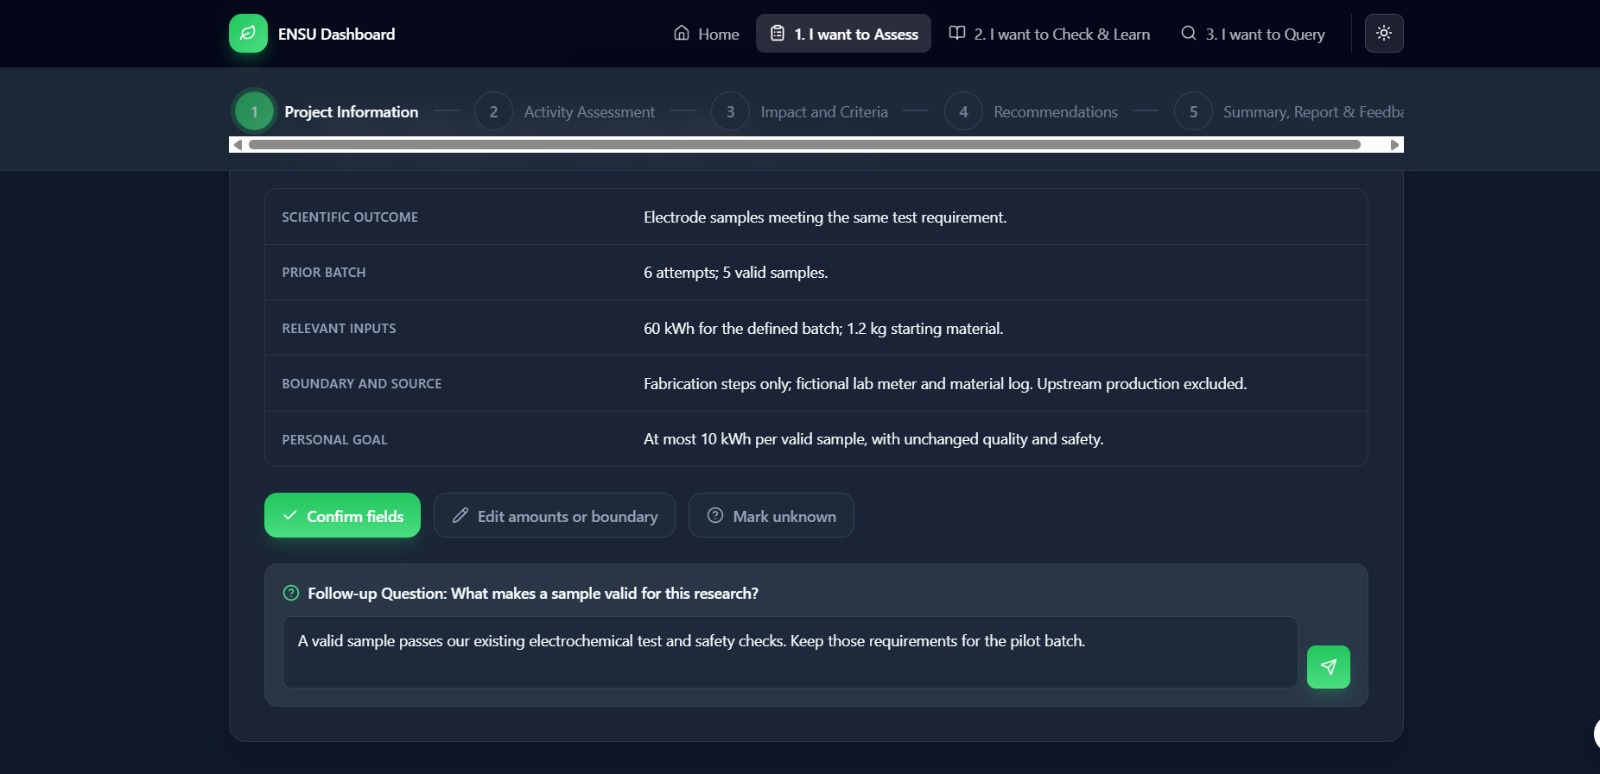
\includegraphics[width=\linewidth,height=0.115\textheight,keepaspectratio]{assets/images/phase2/04-project-information.jpeg}
        \caption{I want to assess - project information}
    \end{subfigure}
    \hfill
    \begin{subfigure}{0.48\linewidth}
        \centering
        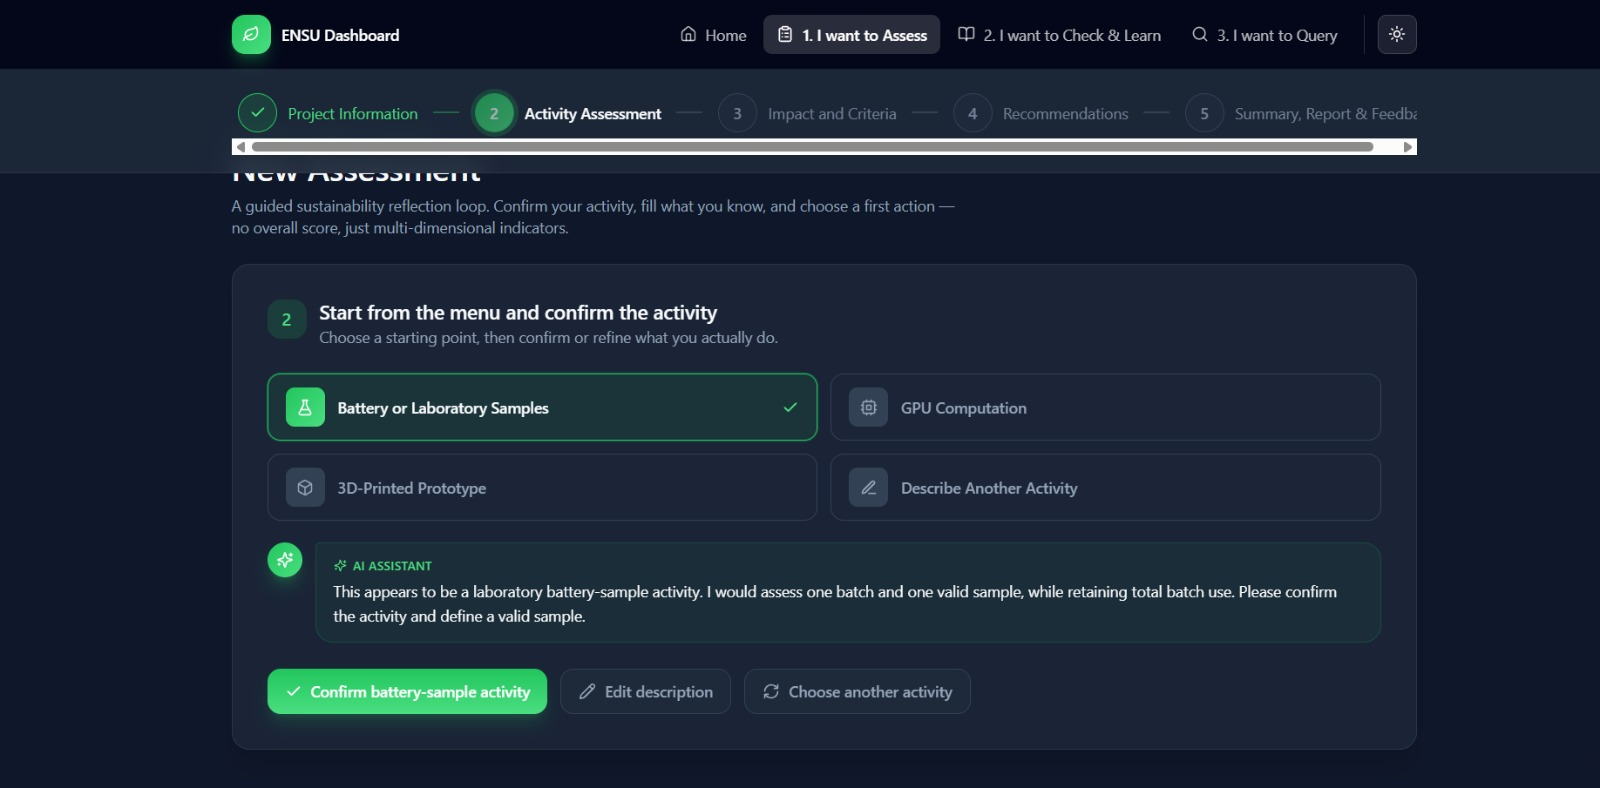
\includegraphics[width=\linewidth,height=0.115\textheight,keepaspectratio]{assets/images/phase2/03-activity-assessment.jpeg}
        \caption{I want to assess - activity assessment}
    \end{subfigure}
    
    \vspace{0.12cm}

    % Row 3
    \begin{subfigure}{0.48\linewidth}
        \centering
        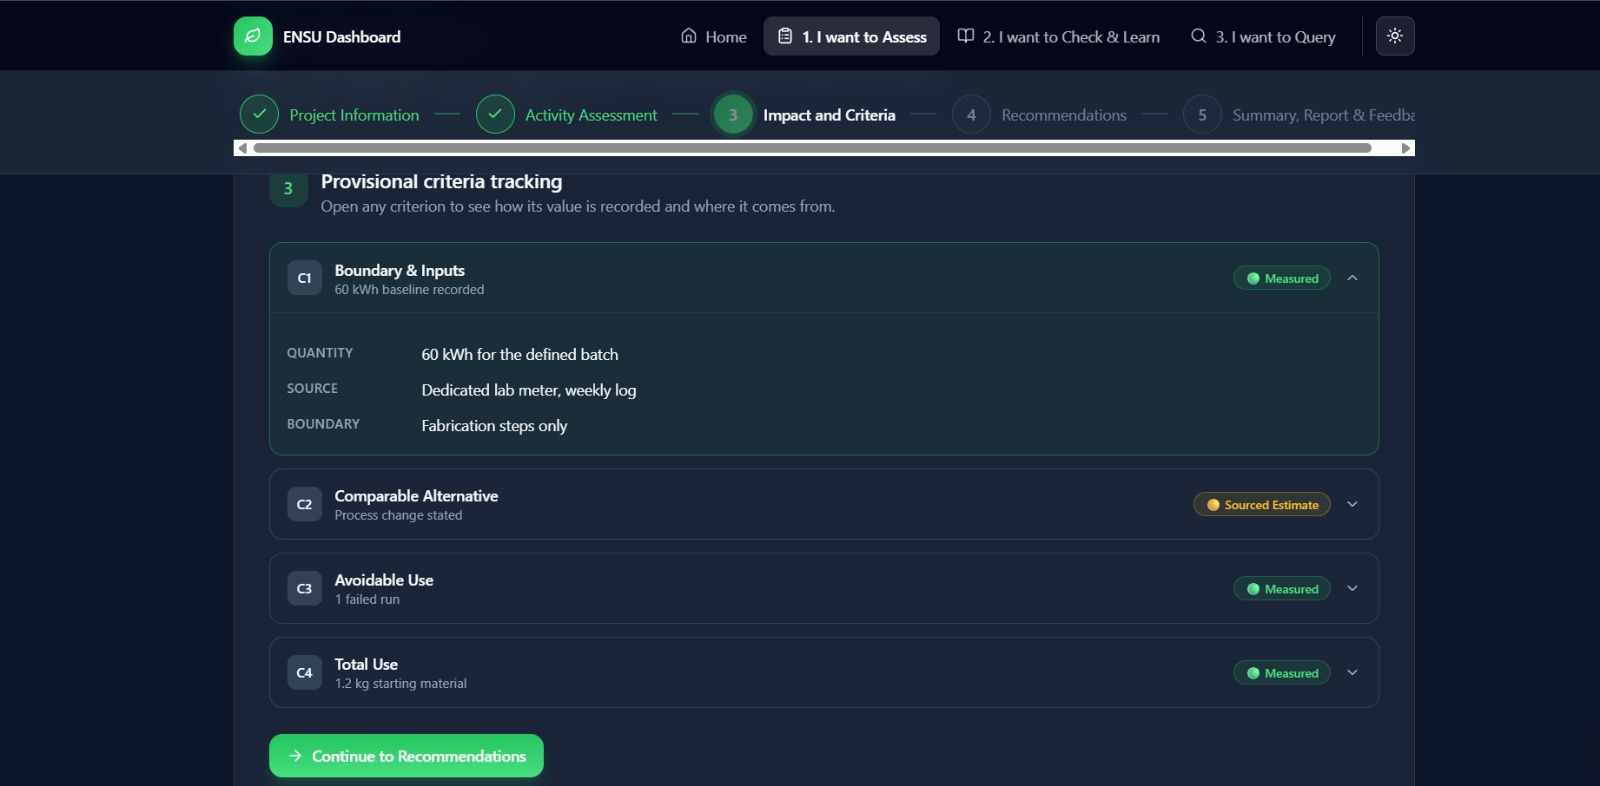
\includegraphics[width=\linewidth,height=0.115\textheight,keepaspectratio]{assets/images/phase2/05-impact-and-criteria.jpeg}
        \caption{I want to assess - impact and criteria}
    \end{subfigure}
    \hfill
    \begin{subfigure}{0.48\linewidth}
        \centering
        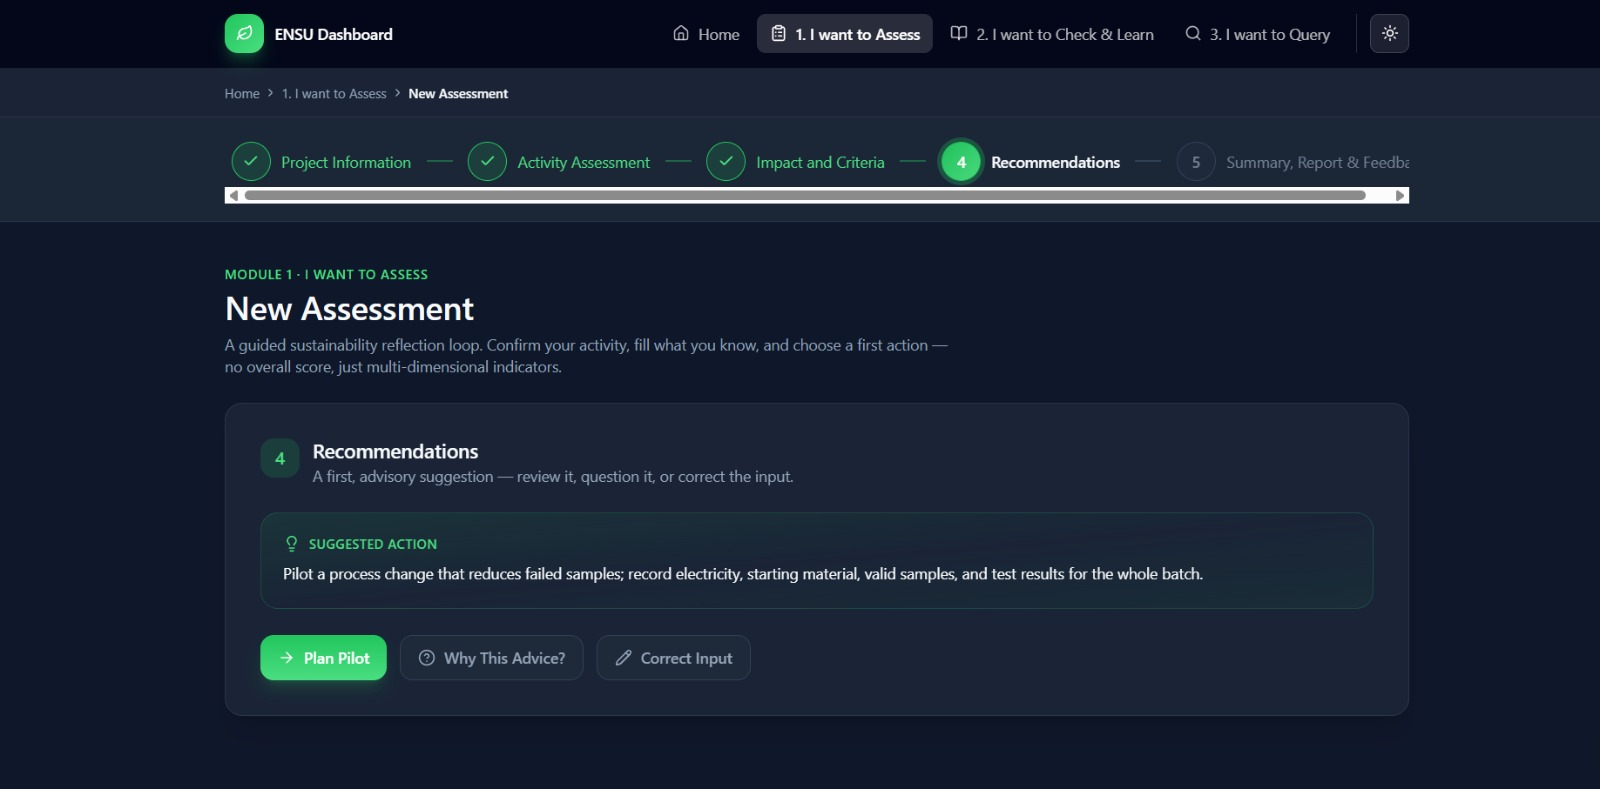
\includegraphics[width=\linewidth,height=0.115\textheight,keepaspectratio]{assets/images/phase2/10-recommendations.jpeg}
        \caption{I want to assess - recommendations}
    \end{subfigure}
    
    \vspace{0.12cm}

    % Row 4
    \begin{subfigure}{0.48\linewidth}
        \centering
        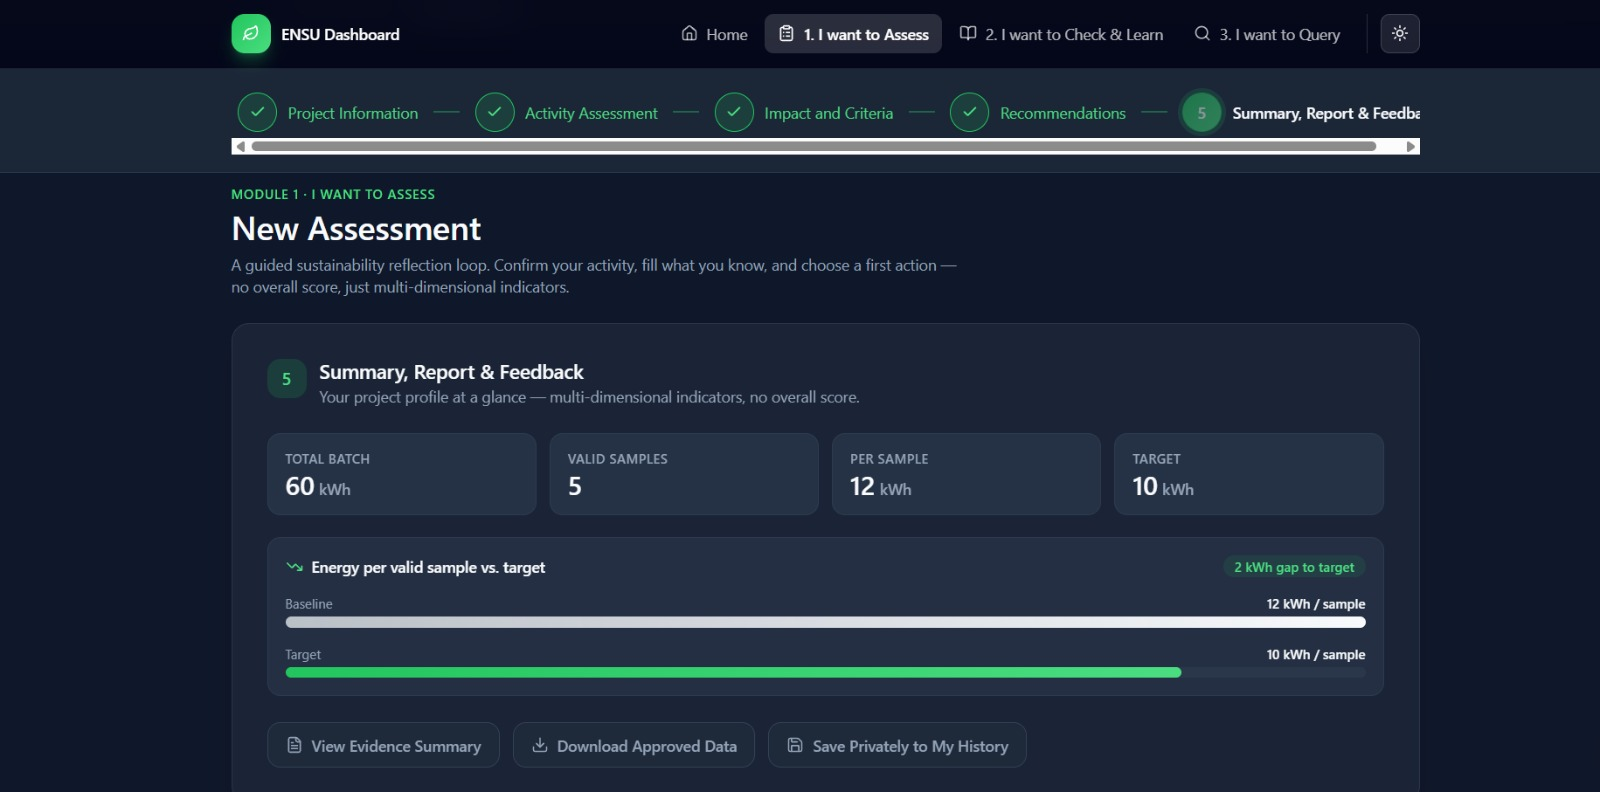
\includegraphics[width=\linewidth,height=0.115\textheight,keepaspectratio]{assets/images/phase2/09-summary-and-feedback.jpeg}
        \caption{I want to assess - summary, report \& feedback}
    \end{subfigure}
    \hfill
    \begin{subfigure}{0.48\linewidth}
        \centering
        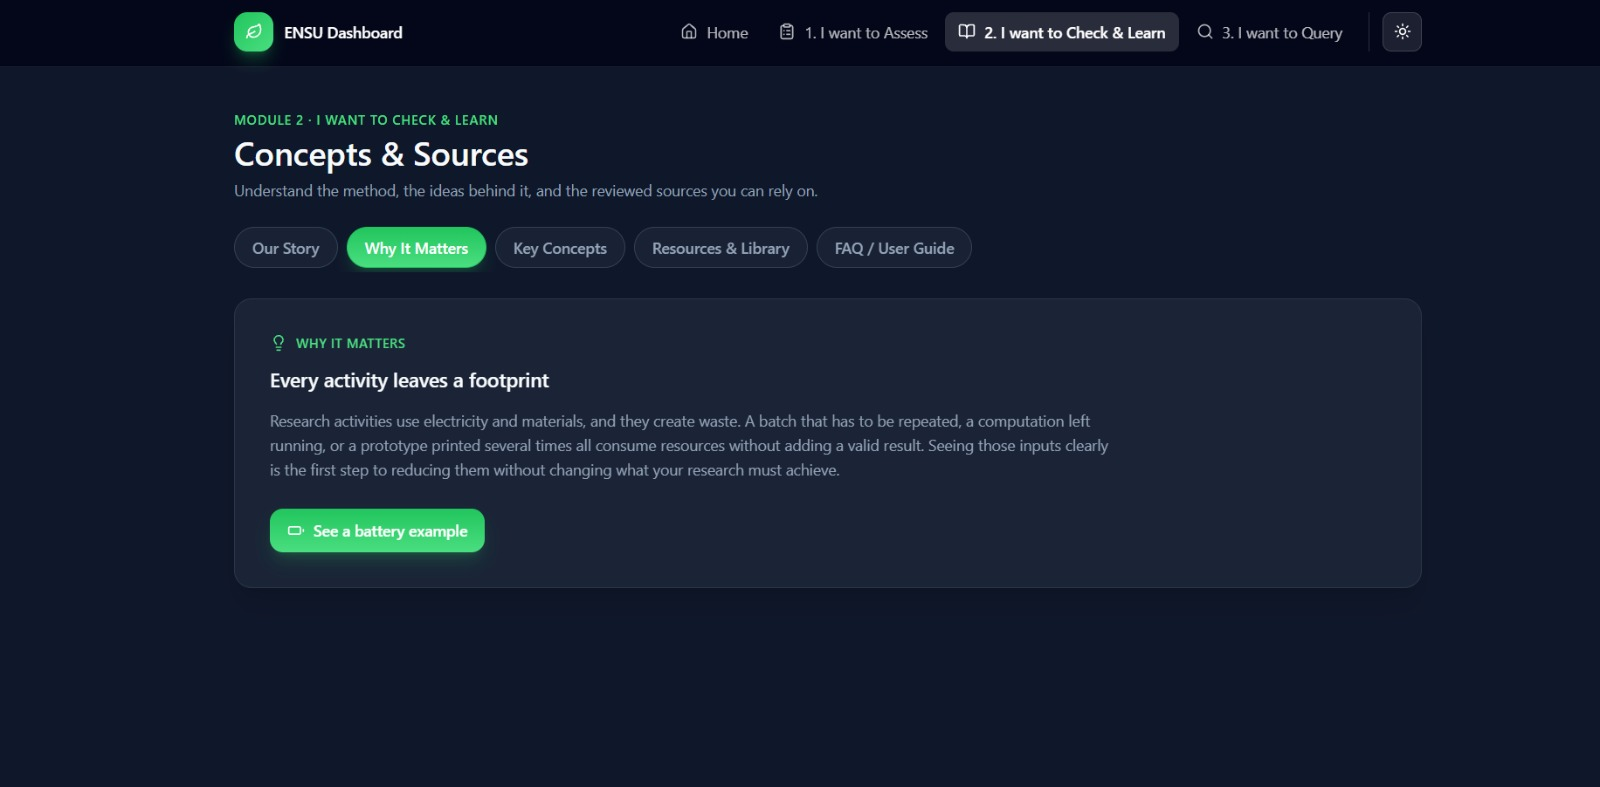
\includegraphics[width=\linewidth,height=0.115\textheight,keepaspectratio]{assets/images/phase2/08-check-and-learn.jpeg}
        \caption{I want to check and learn}
    \end{subfigure}

    \vspace{0.12cm}

    % Row 5
     \begin{subfigure}{0.48\linewidth}
        \centering
        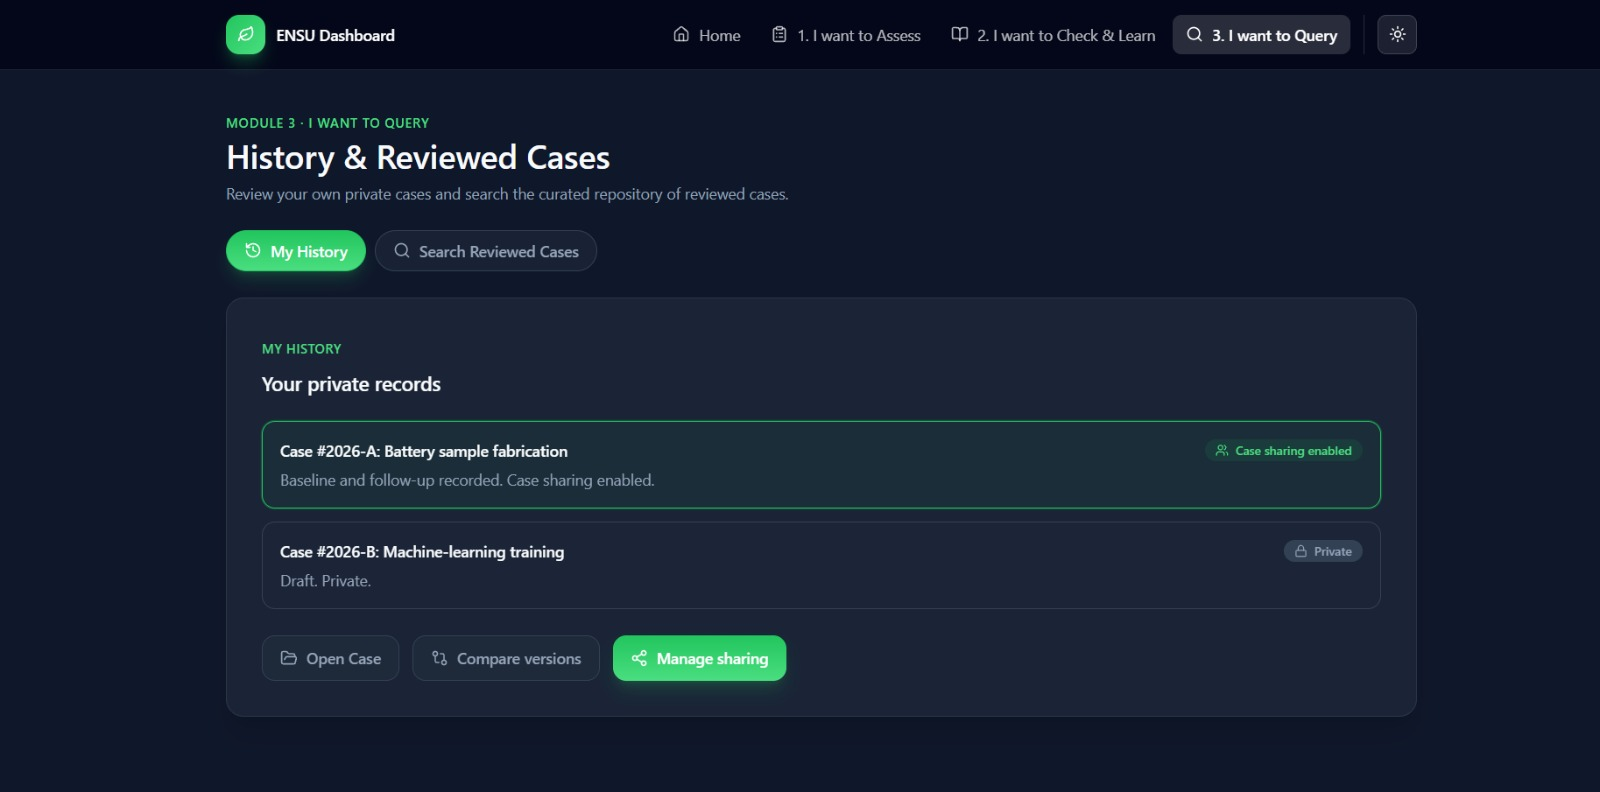
\includegraphics[width=\linewidth,height=0.115\textheight,keepaspectratio]{assets/images/phase2/07-query-dark.jpeg}
        \caption{I want to query - dark mode}
    \end{subfigure}
    \hfill
    \begin{subfigure}{0.48\linewidth}
        \centering
        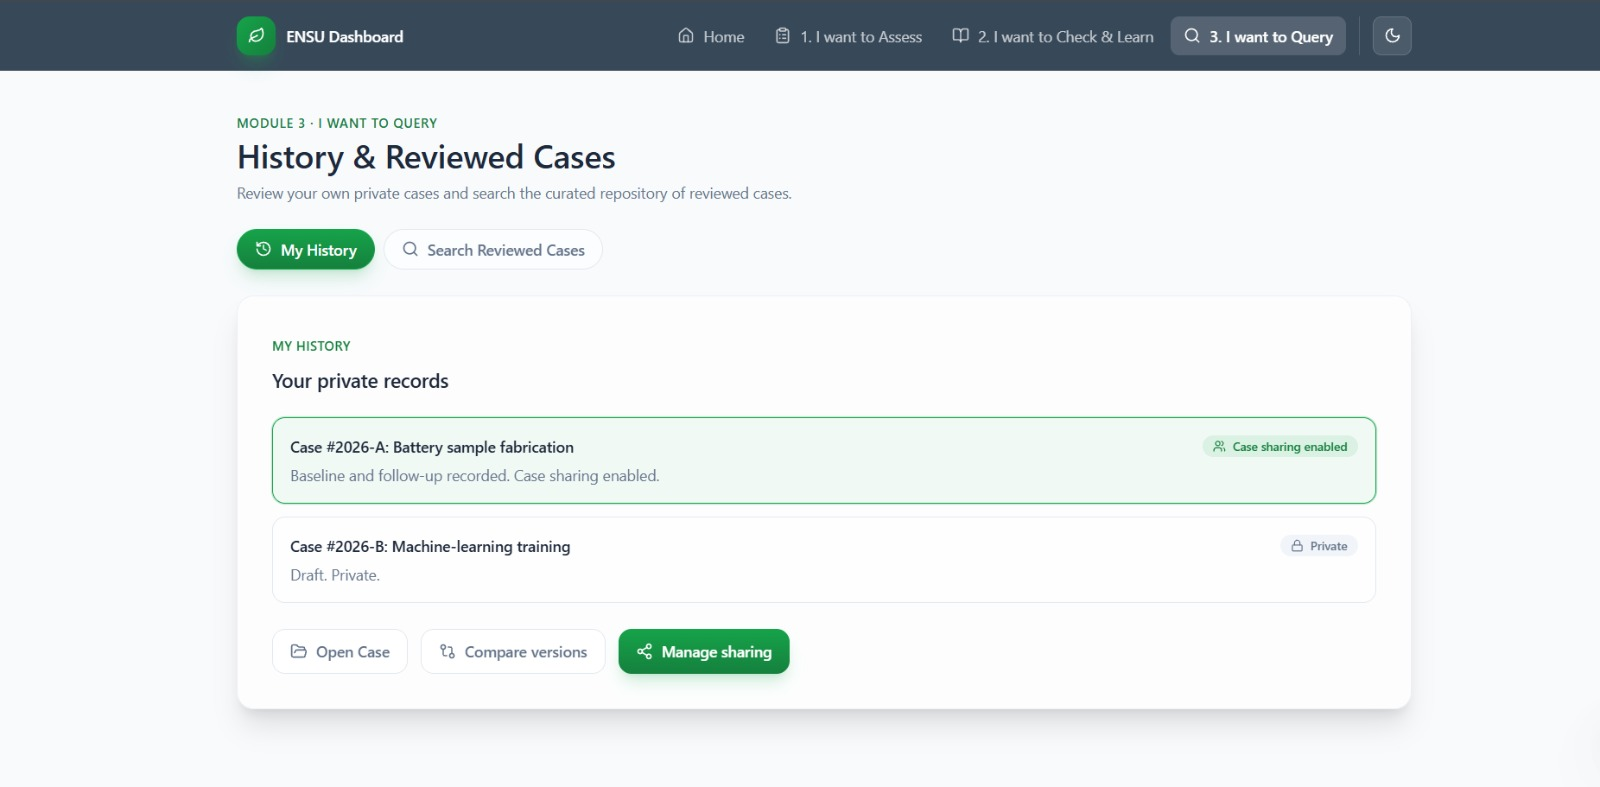
\includegraphics[width=\linewidth,height=0.115\textheight,keepaspectratio]{assets/images/phase2/06-query-light.jpeg}
        \caption{I want to query - light mode}
    \end{subfigure}

    \caption{Earlier self-assessment mock-up corresponding to Section F. The example inputs and outputs illustrate the proposed interaction; they are not measured evaluation results.}
    \label{fig:all_mockups}
\end{figure}
    

\clearpage

% =========================================================================
% H. TECHNICAL DOCUMENTATION & INSTRUCTIONS
% =========================================================================
% AUTHOR TODO -- Gerald coordinates: H is required in the group report; collect actual prompt/source/tool records from every contributor. I/J/K are separate.
\section*{H. Documentation of Prompts, Sources, and Tools}
\addcontentsline{toc}{section}{H. Documentation of Prompts, Sources, and Tools}
%TC:ignore
\noindent\textbf{Contributor completion notes -- Gerald coordinates.}
These are handover requirements, not a record of completed model or API tests.
\begin{itemize}[leftmargin=*]
\item Collect the actual prompts and refinements used for the demo, with their purpose and any model or tool version recorded by the contributor.
\item Identify which sources were actually queried or imported. Distinguish documentation review from successful API access, and illustrative records from retrieved records.
\item Give the real steps needed to reproduce the demo: inputs, source preparation, retrieval, output inspection and correction. Record known failures and missing dependencies.
\item Document current files and editing tools. The report is maintained in \texttt{Phase2.tex}; its embedded bibliography is edited in that file. Run \texttt{scripts/compile.ps1 -Document Phase2} from the project workspace to build \texttt{output/pdf/Phase2.pdf}.
\item For the written report, document AI-assisted drafting, restructuring, language editing and source checking of B/C and the editorial notes. Add the other contributors' actual tool use; do not label this work as spelling correction alone.
\end{itemize}
%TC:endignore

% =========================================================================
% APPENDIX / REMINDERS FOR SEPARATE SUBMISSIONS (Optional Section)
% =========================================================================
\iffalse
\section*{Separate Evaluation Deadlines (Do Not Include in Main Paper PDF)}
The following elements are tracked by the course syllabus but must be submitted through their individual portals independently:
- I. Video/Oral Pitch (3-5 minutes)
- J. Personal Reflection (500 words per student)
- K. Peer Evaluation Sheet
\fi


%TC:ignore
\clearpage
\section*{Editorial checklist -- remove before submission}
\noindent\textbf{Team working notes, excluded from section word counts.}

\subsection*{Section C -- revision completed for team review}
\begin{itemize}[leftmargin=*]
\item The two trees, knowledge-boundary metaphor and module-level replication choice now form one design argument. Sources support the methods; effectiveness is not claimed as a measured result.
\item Cold start now separates initial collection coverage from users without publications. Pure import is permission-dependent and optional; booking inference is deferred.
\item Deployment now distinguishes hosting, authentication, application permissions and Pure identity mapping. Proposed TU/e arrangements are not represented as secured approvals.
\item Peer feedback is addressed through contact preferences, a concrete confidentiality conflict, withdrawal boundaries, correction handling and resource comparisons. Dennis should develop the ethical justification in D without duplicating C's workflow description.
\end{itemize}

\subsection*{Section D -- Dennis}
\begin{itemize}[leftmargin=*]
\item Retain the source-transparency and coverage measures. Review the minor terminology change from chatbot to interface; confirm whether a chatbot remains part of the design.
\item Work through a specific conflict between discovering reusable resources and protecting unpublished ideas. Use the course framework to identify affected parties, compare options, justify a choice and define a review process.
\item Specify contact preferences and the separation between using the tool and sharing a research summary.
\item Explain withdrawal for live records, derived indexes, saved results and external copies; distinguish voluntarily shared summaries from independently public publications.
\item Explain how incorrect links are flagged, checked, corrected and retested. A rejected suggestion is not automatically a reliable training label.
\item Link researcher autonomy to replication choices and to the right to disregard suggestions. Consider users and departments with sparse records.
\end{itemize}

\subsection*{Remaining components -- Gerald coordinates}
\begin{itemize}[leftmargin=*]
\item \textbf{A/B:} Confirm one product name across report and pitch. B has been updated to the current tool; confirm the wording against the final interface and shared example. Its maximum remains 150 words.
\item \textbf{E:} Check each source against the claim it supports, as well as author names, dates, identifiers and reference style. Add sources only after consulting them. The eleven revised C references have received independent source checking; any new source added by a contributor also needs verification.
\item \textbf{F:} Replace the legacy batch-calculation story with a concrete current journey: location, input, source-backed tree output, researcher decision and sharing choice; maximum 500 words.
\item \textbf{G:} Replace the old screenshots with one readable A4 page matching F. Include sample input/output, two trees and a legible source card. Clearly distinguish illustrative output from actual retrieved results.
\item \textbf{H:} Collect actual prompts, sources, model/tool versions where known, explored steps, limitations and reproducible hand-off instructions from the group. Replace every placeholder. Keep proposed integrations separate from completed work; disclose AI assistance accurately.
\item \textbf{I:} Submit the 3--5 minute pitch separately. \textbf{J/K:} Each member submits the personal reflection and peer evaluation separately. These are not additional sections to write in this group PDF, but they are not automatically optional.
\item \textbf{Final check:} Recount B/C/D/F, remove this checklist, update the draft status only when accurate, compile and inspect all pages, and verify the uploaded file and submission receipt.
\end{itemize}
%TC:endignore

\end{document}
